\documentclass[twocolumn,a4paper]{article}
\usepackage{graphicx}
\usepackage[latin1]{inputenc}
\usepackage{amssymb,amsmath,array}
\usepackage{eusflat2013}
\usepackage{lmodern} % Times fonts
\usepackage{amsthm}
\usepackage{multirow}

\hyphenation{pro-per-ties}
\hyphenation{ge-ne-ral-ly}
\hyphenation{pre-fe-ren-ces}
\hyphenation{u-sing}
\hyphenation{pu-nish-ment}

\newcommand{\Pow}{\mathcal{P}}
\newcommand{\N}{\operatorname{N}}
\newcommand{\bool}{\operatorname*{\mathcal{B}}}
\newcommand{\Pos}{\operatorname{Pos}}
\newcommand{\Nec}{\operatorname{Nec}}
\newcommand{\Open}{\operatorname{Open}}
\newcommand{\Rp}{\operatorname{Rp}}
\newcommand{\Rn}{\operatorname{Rn}}
\newcommand{\FB}{\operatorname{FB}}
\newcommand{\UC}{\operatorname{UC}}
\newcommand{\T}{\mathcal{T}}
\newcommand{\Rel}{\mathcal{R}}
\newcommand{\C}{\mathcal{C}}
\newcommand{\Boolean}{\mathbb{B}}
\newcommand{\Nat}{\mathbb{N}}
\newcommand{\Q}{\mathbb{Q}}
\newcommand{\R}{\mathbb{R}}
\newcommand{\Z}{\mathbb{Z}}
\newcommand{\Head}{\mathcal{H}}
\newcommand{\Body}{\mathcal{B}}
\newcommand{\Dom}{\mathcal{D}}
\newcommand{\INS}{\mbox{\textbf{insert}}}
\newcommand{\DEL}{\mbox{\textbf{delete}}}
\newcommand{\MOD}{\mbox{\textbf{modify}}}
\newcommand{\REV}{\mbox{\textbf{revise}}}
\newcommand{\AR}{\mbox{\textbf{ AR }}}
\newcommand{\Overlap}{\mbox{\textbf{Overlap}}}
\newcommand{\A}{\mathcal{A}}
\newcommand{\I}{\mathcal{I}}
\newcommand{\M}{\mathcal{M}}
\renewcommand{\Join}{\bowtie}
\theoremstyle{definition}
\newtheorem{definition}{Definition}
\newtheorem{example}{Example}

%***********************************************************************
% !!!! IMPORTANT NOTICE ON TEXT MARGINS !!!!!
%***********************************************************************
%
% Please avoid using DVI2PDF or PS2PDF converters: some undesired
% shifting/scaling may occur when using these programs
% It is strongly recommended to use the DVIPS converters, and to submit
% PS file. You may submit a PDF file if and only if you use ADOBE ACROBAT
% to convert your PS file to PDF.

%\setlength\paperheight{297mm}
%\setlength\paperwidth{210mm}


%***********************************************************************
% !!!! USE OF THE Atlantis Press LaTeX STYLE FILE !!!!!
%***********************************************************************
%
% Some commands are inserted in the following .tex example file.  Therefore to
% set up your Atlantis Press submission, please use this file and modify it to insert
% your text, rather than staring from a blank .tex file.  In this way, you will
% have the commands inserted in the right place.




\begin{document}

\title{A Comparison of Approaches to Model Uncertainty in Time Intervals}

\begin{aug}
\author[1]{Christophe Billiet}
\author[2]{Jos\'{e} Enrique Pons}
\author[2]{Olga Pons Capote}
\author[1]{Guy de Tr\'{e}}
\affilation[1]{Department of Telecommunications and Information Processing, Ghent University, Belgium.
%\\ Sint-Pietersnieuwstraat 41, B-9000 Ghent, Belgium
}
\affilation[2]{Department of Computer Science and Artificial Intelligence, University of Granada, Spain.
%\\ C/Periodista Daniel Saucedo Aranda s/n E-18071 (Granada-Spain)
}
\end{aug}


\maketitle
\thispagestyle{empty}

\begin{abstract}
Information systems model parts of reality by representing properties of real-world objects or concepts. As real objects or concepts often have temporal aspects, temporal notions such as time intervals are often represented. However, these may contain imperfections like uncertainties, complicating their representations. A very important purpose of information systems is to be able to query them to retrieve information, but representations of temporal notions containing uncertainties severely complicate querying. Thus, several soft computing techniques have been proposed to represent time intervals subject to uncertainties in a semantically sound way and to reason with them in a semantically sound and useful way. In the presented work, two frameworks designed for this are compared. It is found that, despite slight differences in the way these frameworks represent intervals, they provide the same results when reasoning about time intervals subject to uncertainty.
\end{abstract}

\begin{keywords}
temporal representation, temporal reasoning, possibility theory, information systems, information retrieval, ill-known intervals, uncertainty
\end{keywords}

\section{\label{sec:introduction}Introduction}
Information systems (IS) have always tried to model parts of reality. To achieve this modelling, such systems contain data representing properties of real-world objects or concepts~\cite{JoseEnriquePons2012},~\cite{Billiet2012}. As time is an essential aspect of many real-world objects or concepts, information systems often contain data representing temporal notions which describe such temporal properties~\cite{Bolour1982},~\cite{VanderCruyssen1997}. Such temporal notions usually take the form of either instants~\cite{Jensen1998}, which can informally be seen as infinitely short `moments' or `points' in time, or time intervals~\cite{Jensen1998}.

Data are often produced by humans, but human-made data are prone to imperfections: some data may be vague, imprecise, incomplete, contradictory or uncertain. Data representing temporal notions may contain such imprecisions too~\cite{Devos1994},~\cite{Dubois2003},~\cite{JoseEnriquePons2012},~\cite{Billiet2012}. The work presented in this paper is specifically concerned with time intervals (and as a special case: instants) subject to uncertainty.

Generally, one of the most important purposes of an IS is to allow the retrieval of information or knowledge deduced from its data. Information or knowledge is usually retrieved from an IS by querying it and examining or analyzing the query results or by visualizing the contents of the IS, querying this visualization and examining or analyzing the resulting visualization(s).

Of course, when temporal information is represented in an IS, querying this IS may have a temporal aspect too. Usually, querying an IS containing data representing temporal notions is conceptually done by specifying one or more time indications and requesting information that is in a specific relationship with these indications, where the semantics of these relationships are specifically temporal~\cite{Billiet2012},~\cite{JoseEnriquePons2012},~\cite{Pons2012a}. Thus, some existing proposals have considered groups of basic relationships between time indications used to construct and express specific temporal relationships~\cite{Medina1994},~\cite{Schockaert2008}. Notably, Allen~\cite{Allen1983} presented a reasoning framework containing all semantically usefull basic temporal relationships between time intervals (and as a special case instants). The resulting relationships are shown in figure \ref{fig:allen-relationships}. These Allen relationships are used in the presented work.

\begin{figure}[h]
   \centering
   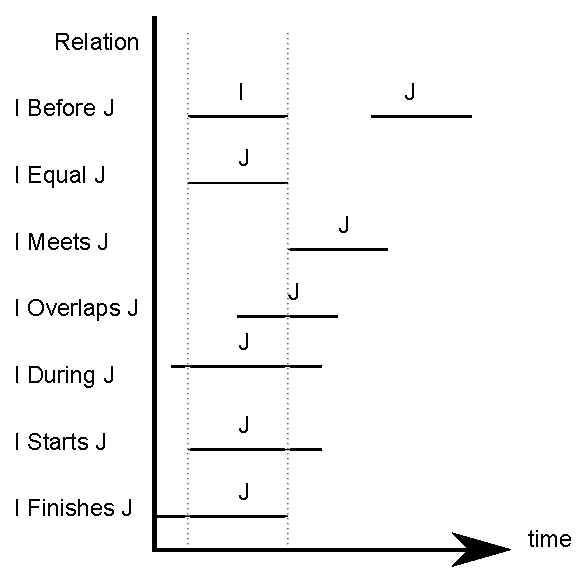
\includegraphics[width=0.9\columnwidth]{graphs/allen.eps}
   \caption{The Allen relationships between two crisp intervals $I$ and $J$.  }
   \label{fig:allen-relationships}
 \end{figure}

To be able to query IS containing data representing time indications subject to uncertainty, a framework is necessary, able to represent uncertainties in time indications in a semantically sound way, without (much) information loss and able to temporally reason with such time indications in a semantically sound and usefull way~\cite{Dubois1983},~\cite{Dubois2003}. Although more proposals for such frameworks exist, the work presented in this paper focusses on just two: the \emph{ill-known constraint \emph{(IKC)} framework}~\cite{Pons2011} and the \emph{triangular model \emph{(TM)} framework}~\cite{DeTre2012}.

The work presented in this paper consists of a comparison of both frameworks, about the approaches they use to represent time intervals subject to uncertainty and to reason about the temporal relationships between such intervals and time intervals without uncertainty.

The structure of this paper is as follows: section \ref{sec:general-preliminaries} presents some general preliminaries and naming and notation conventions used in this paper. Sections \ref{sec:ikc} and \ref{sec:tm} introduce the IKC and TM frameworks respectively: both sections first introduce some preliminary concepts and techniques specific to the framework under consideration, then explain how the representation of time intervals by the framework is done and finally show how the evaluation of Allen relationships between an interval subject to uncertainty and one without uncertainty is done. In section \ref{sec:proposal}, both frameworks are compared: first their approaches to representing time intervals are compared, next their approaches to evaluating Allen relationships are compared. Finally, section \ref{sec:conclusions} presents the principal conclusions of the presented work and some possible future work. 

%TODO: more references in the above part?
%TODO: include some form of proof or previous work with these statements?!

%The concept of the time has been widely studied \cite{Benthem1982}, \cite{Shackle1961}, \cite{Klein1994}. Moreover, humans beings manage temporal indications in an imprecise way \cite{Devos1998}. But when dealing with time in an Information System, some simplifications must to be done. The first thing to do is the discretization of the time line into time points or time intervals. Both approaches have been proved to be equivalent, although due to the nature of the smallest unit of time in a computer, a \emph{chronon}, the discretization of a time point returns a time interval.

%All the possible positions between two time intervals were studied by Allen \cite{Allen1983}, \cite{Allen1985}. As result, the thirteen Allen's Relations were obtained (See Table \ref{tab:allen-relations}) which are illustrated in Figure \ref{fig:allen-relationships}. In order to achieve a more intelligent processing of time, some theoretical frameworks are used to reason with time. First the possibility theory was employed in the reasoning with temporal information \cite{Dubois2003a}. Then, several proposals \cite{Schockaert2008}, \cite{nagypal2003}, \cite{Ohlbach2004}, \cite{Pons2011} studied how to extend the thirteen Allen's relations to the possibilistic case. Also rough set theory \cite{Pawlak1995} has been used to represent and reason about imperfect time intervals \cite{Qiang2009}, \cite{Qiang2010}.

%Although there exists several proposals to represent and visualize imperfect time intervals, in this paper we will focus on two: the ill-known constraint framework \cite{Pons2011} and the triangular model \cite{DeTre2012}. The first one is a theoretical framework that deals with temporal reasoning and the second one is a visual framework that represent imperfect time intervals in a two dimensional space. Both frameworks can be used to represent imperfect time intervals as well as temporal reasoning.

%The structure of this paper is the following. Section  \ref{sec:preliminaries} introduces the Ill-known constraint framework. Section \ref{sec:triangular-model} introduces the triangular model. Section \ref{sec:proposal} analyze both frameworks and shows the correspondences and differences between both frameworks. The section concludes with an example showing that the calculations made in both frameworks are equivalent. Finally, Section \ref{sec:conclusions} presents the main conclusions and the future work. 


%\begin{table}[h]
%\centering
%\begin{tabular}{|c|l|}
%\hline
%Name & Implementation \\ \hline 
%$I$ equals $J$ & if $s_i = s_j \wedge e_i = e_j $ \\
%$I$ starts $J$ & if $s_i = s_j \wedge e_i < e_j $ \\
%$I$ started by $J$ & if $s_i = s_j \wedge e_i > e_j $ \\
%$I$ finishes $J$ & if $s_i > s_j \wedge e_i = e_j $ \\
%$I$ finished by $J$ & if $s_i < s_j \wedge e_i = e_j $ \\
%$I$ meets $J$ & if $e_i = s_j $ \\
%$I$ met by $J$ & if $s_i = e_j $ \\
%$I$ overlaps $J$ & if $s_i < s_j \wedge e_i < e_j \wedge e_i > s_j $ \\
%$I$ overlapped by $J$ & if $s_i > s_j \wedge e_j < e_i \wedge s_i < e_j  $ \\
%$I$ during $J$ & if $s_i > s_j \wedge e_i < e_j $ \\
%$I$ contains $J$ & if $  s_i < s_j \wedge e_i > e_j$ \\
%$I$ before $J$ & if $e_i < s_j $ \\
%$I$ after $J$ & if $s_i > e_j $ \\
%\hline
%\end{tabular}
%\caption{Allen's relations represented in the framework. $I = \left[s_i, e_i\right]$, $J=  \left[s_j, e_j\right]$}
%\label{tab:allen-relations}
%\end{table}



\section{\label{sec:general-preliminaries}General Preliminaries, Notations and Nomenclature}
Often, time is thought of as following an axis (a time axis) and thus it is often seen as an ordered set of infinitely short `moments' or `points' in time, called \emph{instants}~\cite{Dyreson1994},~\cite{Jensen1998}. This is also the case in the presented work. A \emph{time interval} is then an interval subset of this ordered set of instants. In this paper, instants are noted using lowercase letters and time intervals using uppercase letters. Also, a time interval $I$ starting at (and containing) instant $s$ and ending at (and containing) instant $e$ is noted using square brackets: $I = \left[s, e\right]$.

The presented work allows time intervals to be subject to uncertainties. These uncertainties are always seen as caused by a (partial) lack of knowledge: the exact, intended time interval is not known, eventhough there is only one correct intended time interval and as such no variability. Confidence about exactly which interval is the intended one in the context of such uncertainties is modelled using possibility theory~\cite{DidierDubois1988a}. In the presented work, possibility is always interpreted as plausibility given a (partial) lack of knowledge.

To be able to distinguish easily, time intervals not subject to uncertainties will be called \emph{crisp time intervals} in the presented work.

\section{\label{sec:ikc}The Ill-known Constraint Framework}
\documentclass[10pt,a4paper]{article}
\usepackage[latin1]{inputenc}
\usepackage{amsmath}
\usepackage{amsfonts}
\usepackage{amssymb}
\usepackage{graphicx}


\hyphenation{pro-per-ties}
\hyphenation{ge-ne-ral-ly}
\hyphenation{pre-fe-ren-ces}
\hyphenation{u-sing}
\hyphenation{pu-nish-ment}

\newcommand{\Pow}{\mathcal{P}}
\newcommand{\N}{\operatorname{N}}
\newcommand{\bool}{\operatorname*{\mathcal{B}}}
\newcommand{\Pos}{\operatorname{Pos}}
\newcommand{\Nec}{\operatorname{Nec}}
\newcommand{\T}{\mathcal{T}}


\author{Jose Enrique}
\title{Possibility and necessity for each Ill-known Constraint}
\begin{document}
Implementation of the ill-known constraints:
We will consider the following elements:
\begin{itemize}
\item $X$ an ill-known value.
\item $[D,c,e]$ a triangular possibility distribution. Where the core is $D$ and $D-c$ is the lower bound, $D+e$ is the higher bound.
\item $I = [a, b]$ a crisp interval where $a$ is the starting point and $b$ is the ending point.
\end{itemize}


\section*{$C\triangleq(\leq,X)$}
\begin{align}
\Pos (C([a,b])) &= \min_{r \in [a,b]} \sup_{\omega \leq r} \pi_X(\omega) = \\
\Pos (C([a,b])) &= \sup_{\omega \leq a} \pi_X(\omega)
\end{align}

So, for $I=[a,b]$ and  $X=[D,c,e]$ we have:

\begin{equation}
Pos (C[a,b]) = \mu_{\leq}(a) =
\begin{cases}
1 & \mbox{ if } a \leq D \\
\frac{a-(D+e)}{e} & \mbox{ if } a > D \wedge a < (D+e) \\
0 & \mbox{ otherwise }
\end{cases}
\end{equation}


\begin{figure}[h]
\centering
\includegraphics[scale=1]{graphs/lte.pdf}
\end{figure}



\section*{$C\triangleq(<,X)$}
\begin{align}
\Pos (C([a,b])) &= \min_{r \in [a,b]} \sup_{\omega < r} \pi_X(\omega) = \\
\Pos (C([a,b])) &= \sup_{\omega < a} \pi_X(\omega)
\end{align}

\begin{equation}
Pos (C[a,b]) = \mu_{<}(a) =
\begin{cases}
1 & \mbox{ if } a < (D-c) \\
\frac{a-D}{c} & \mbox{ if } a \geq (D-c) \wedge a \leq D \\
0 & \mbox{ otherwise }
\end{cases}
\end{equation}

\begin{figure}[h]
\centering
\includegraphics[scale=1]{graphs/lt.pdf}
\end{figure}


\section*{$C\triangleq(\geq,X)$}
\begin{align}
\Pos (C([a,b])) &= \min_{r \in [a,b]} \sup_{\omega \geq r} \pi_X(\omega) = \\
\Pos (C([a,b])) &= \sup_{\omega \geq b} \pi_X(\omega)
\end{align}
\begin{figure}[h]
\centering
\includegraphics[scale=1]{graphs/gte.pdf}
\end{figure}

\begin{equation}
Pos (C[a,b]) = \mu_{\geq}(b) =
\begin{cases}
1 & \mbox{ if } b \geq D \\
\frac{(D-c)-b}{c} & \mbox{ if } a \geq (D-c) \wedge a \leq D \\
0 & \mbox{ otherwise }
\end{cases}
\end{equation}



\section*{$C\triangleq(<,X)$}
\begin{align}
\Pos (C([a,b])) &= \min_{r \in [a,b]} \sup_{\omega > r} \pi_X(\omega) = \\
\Pos (C([a,b])) &= \sup_{\omega > b} \pi_X(\omega)
\end{align}


\begin{equation}
Pos (C[a,b]) = \mu_{<}(b) =
\begin{cases}
1 & \mbox{ if } b \geq (D+e) \\
\frac{D-b}{e} & \mbox{ if } a \geq (D-c) \wedge a \leq D \\
0 & \mbox{ otherwise }
\end{cases}
\end{equation}

\begin{figure}[h]
\centering

\includegraphics[scale=1]{graphs/gt.pdf}
\end{figure}


\section*{$C\triangleq(=,X)$}
\begin{align}
\Pos (C([a,b])) = \min_{r \in [a,b]} \sup_{\omega = r} \pi_X(\omega)
\end{align}
\begin{figure}[h]
\centering
\includegraphics[scale=1]{graphs/eq.pdf}
\end{figure}

\section*{$C\triangleq(\neq,X)$}
\begin{align}
\Pos (C([a,b])) = \min_{r \in [a,b]} \sup_{\omega \neq r} \pi_X(\omega)
\end{align}
\begin{figure}[h]
\centering
\includegraphics[scale=1]{graphs/neq.pdf}
\end{figure}




\end{document}

\section{\label{sec:tm}The Triangular Model Framework}
In~\cite{Weghe2007}, the TM framework for crisp intervals is introduced, based on~\cite{Kulpa1997}. In~\cite{DeTre2012}, the framework is generalized to allow the representation of and reasoning with time intervals subject to uncertainty. In this section, this generalization's main aspects towards interval representation and Allen relationship evaluation are briefly presented. 

\subsection{\label{subsec:tm-preliminaries}Preliminary Concepts}
In the triangular model framework, the approaches to interval representation and Allen relationship evaluation are closely related to the approach to interval visualization. Usually, different time intervals are visualized as different parallel line segments in the same image plane. However, as this linear approach introduces a few issues, time intervals are visualized as points in the image plane in the TM framework~\cite{DeTre2012},~\cite{Weghe2007}. To achieve this, a horizontal line segment visualizing the used (part of the) time axis is drawn in the image plane (this is called the \emph{time line}). Then, a triangle is drawn, using this line segment as a side of which the angles with the other two sides have sizes $\alpha$ and $-\alpha$ respectively. The area contained in this triangle is called the \emph{interval space} and will contain all visualizations of intervals. Now, the procedure used to visualize a CTI $\left[s, e\right]$ in the interval space is the following~\cite{DeTre2012},~\cite{Weghe2007}:
\vspace{-5pt}
\begin{enumerate}
	\item $s$ is visualized as a point on the time line.
	\item A straight half-line $L_s$ is constructed from this point, having, in this point, an angle of size $\alpha$ with the time line.
	\item $e$ is visualized as a point on the time line.
	\item A straight half-line $L_e$ is constructed from this point, having, in this point, an angle of size $-\alpha$ with the time line.
	\item The intersection point of $L_s$ and $L_e$ is the intended visualization of interval $\left[s, e\right]$.
\end{enumerate}
\vspace{-5pt}
A similar point visualizing an interval is generally called an \emph{interval point}~\cite{DeTre2012},~\cite{Weghe2007}. In this work, as it is usually done, the size of $\alpha$ is chosen to be $45^{\circ}$. An example of such construction is shown in figure \ref{fig:tm-const-ex}.

\begin{figure}[h]
	\centering
	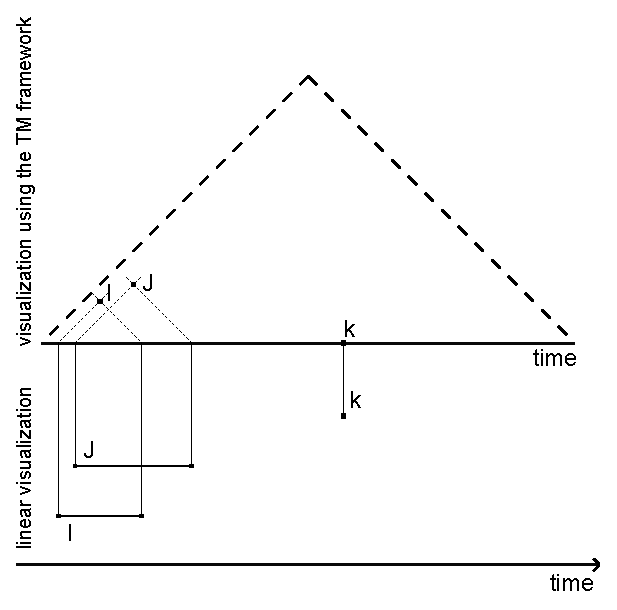
\includegraphics[width=0.9\columnwidth]{graphs/TM_model_several.eps}
	\caption{The visualization of several CTI using the TM framework.}
	\label{fig:tm-const-ex}
\end{figure}
\vspace{-10pt}

\subsection{\label{subsec:tm-interval}Representation of Time Intervals Subject to Uncertainty}
The TM framework allows uncertainty in time intervals by supporting uncertain time intervals~\cite{DeTre2012}:

\begin{definition}
Given an ordered set of instants $T$, an \emph{uncertain time interval} (UTI) $J$ in $T$ is here a time interval defined by a pair
\begin{align}
J \triangleq (\pi_s, \pi_e) \nonumber
\end{align}
where $\pi_s$ and $\pi_e$ are two convex~\cite{Dubois1983} possibility distributions on $T$.
\end{definition}

Consider an ordered set of instants $T$ and an UTI $J$ in $T$, defined by the pair $(\pi_s, \pi_e)$. Given an instant $x \in T$, $\pi_s(x)$ now expresses the possibility that $x$ is the starting instant of $J$ and $\pi_e(x)$ expresses the possibility that $x$ is the ending instant of $J$. Thus, $J$ intends to indicate just one CTI, but it is (partially) unknown exactly which time interval this is. The possibility $\pi_J(I)$ that a given CTI $I = \left[s_i, e_i\right]$ is the exact time interval intended by $J$ can now be uniquely determined by~\cite{DeTre2012}:
\vspace{-5pt}
\begin{align}
\pi_J(I) = \begin{cases}
 \min \left(\pi_s (s_i), \pi_e (e_i) \right), & \mbox{ if } s_i \leq e_i\\
0, & \mbox{ otherwise }
\end{cases}
\end{align}

Now consider an ordered set of instants $T$ and a visualization of this in an image plane, using the TM framework. An UTI $J$ in $T$ defined by a pair $(\pi_s, \pi_e)$ is now visualized as an area in the image plane. This area is constructed as follows: for every CTI $K$ for which the possibility $\pi_J(K)$ of $K$ being the CTI intended by $J$ is higher than zero, the interval point is drawn and is given a color. This color is part of a linear single-color greyscale and its saturation is linearly related to the degree of possibility that $K$ is the CTI intended by $J$. Together, these drawn interval points form the visualization of $J$~\cite{DeTre2012}. An example of such construction is shown in figure \ref{fig:tm-ill-const-ex}. In this figure, a darker color of interval point indicates a higher and a lighter color a lower possibility that the corresponding CTI is the intended interval.

\begin{figure}[h]
	\centering
	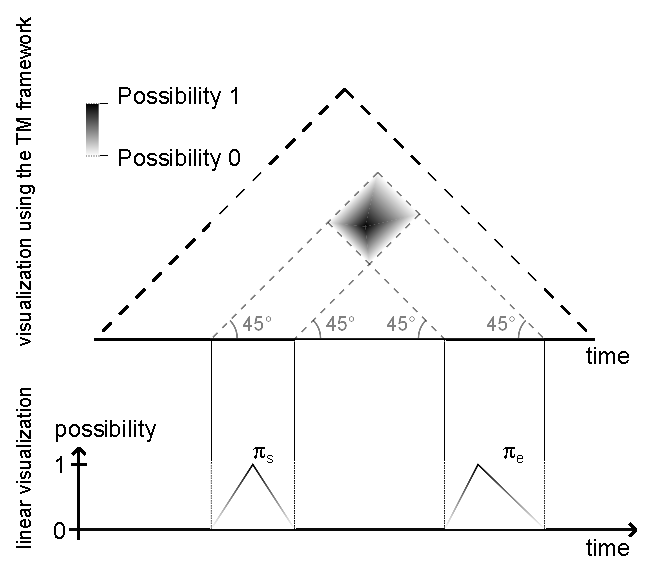
\includegraphics[width=0.9\columnwidth]{graphs/TM_model_ill_known.eps}
	\caption{The visualization of one UTI defined by a pair $(\pi_s, \pi_e)$ using the TM framework.}
	\label{fig:tm-ill-const-ex}
\end{figure}
\vspace{-10pt}

\subsection{\label{subsec:tm-evaluation}Evaluation of Allen Relationships}
At the base of the framework's approach to evaluating Allen relationships is the concept of uncertain relational zones~\cite{DeTre2012}:

\begin{definition}
For a given UTI $J$, the \emph{uncertain relational zones} (URZ) are fixed areas in the interval space.
\end{definition}

Now, given an UTI $J$ and its visualization in an interval space, the procedure to visualize its URZ is the following~\cite{DeTre2012}:

\begin{enumerate}
	\item The visualizations (the points) on the time line of both the smallest and greatest instant with a non-zero possibility of being the starting instant of $J$ are determined.
	\item Two straight half-lines are constructed from each of these points: one having, in the point, an angle of size $\alpha$ with the time line and one having, in the point, an angle of size $-\alpha$ with the time line.
	\item The visualizations (the points) on the time line of both the smallest and greatest instant with a non-zero possibility of being the ending instant of $J$ are determined.
	\item Two straight half-lines are constructed from each of these points: one having, in the point, an angle of size $\alpha$ with the time line and one having, in the point, an angle of size $-\alpha$ with the time line.
	\item The lines constructed this way divide the interval space in at most fifteen different areas, including the area corresponding to the visualization of $J$ itself. These areas are the intended visualizations of $J$'s URZ.
\end{enumerate}

In this procedure, $\alpha$ is the same angle size as in the procedure for the visualization of CTI. The results of this procedure for an example UTI $J$ (as wel as the visualization of $J$ itself) are shown in figure \ref{fig:tm-urz}. 

\begin{figure}[h]
	\centering
	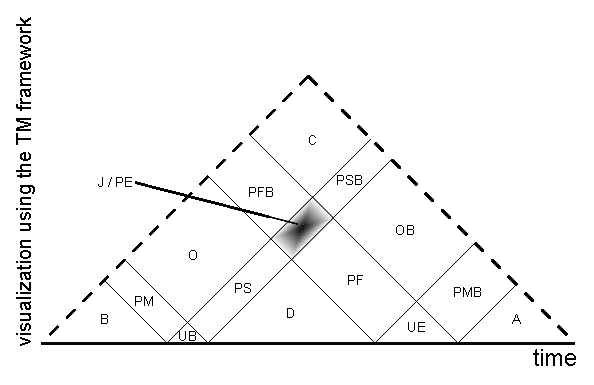
\includegraphics[width=0.9\columnwidth]{graphs/TM_model_URZ.eps}
	\caption{The visualization of the URZ for a given UTI $J$, using the TM framework.}
	\label{fig:tm-urz}
\end{figure}

Given an UTI $J$ and its URZ, every URZ is assigned a symbol and a name and corresponds to a set of Allen relationships~\cite{DeTre2012}. These symbols and names are used to uniquely identify each of $J$'s URZ. The set of Allen relationships corresponding to an URZ contains every Allen relationship in which any interval visualized by one of the URZ's interval points could be with the interval intended by $J$, depending on exactly which CTI $J$ actually intends to represent. In figure \ref{fig:tm-urz}, the URZ's symbols are noted inside the areas visualizing their respective URZ's. In table \ref{tab:urz}, every different row corresponds to a different URZ. In the first two columns, the symbol and name of the URZ are given, the last column contains the set of corresponding Allen relationships. For these, the following notations are used:

\begin{itemize}
	\item `E' denotes `equals'.
	\item `S' denotes `starts'.
	\item `SB' denotes `started by'.
	\item `F' denotes `finishes'.
	\item `FB' denotes `finished by'.
	\item `M' denotes `meets'.
	\item `MB' denotes `met by'.
	\item `O' denotes `overlaps'.
	\item `OB' denotes `overlapped by'.
	\item `D' denotes `during'.
	\item `C' denotes `contains'.
	\item `B' denotes `before'.
	\item `A' denotes `after'.
\end{itemize}
\vspace{-10pt}
\begin{table}[h]
\centering
\begin{tabular}{|l|l|l|}
\hline
Symbol & Name & Relationships \\
\hline
B    & Before & B \\
O    & Overlaps & O \\
C    & Contains & C \\
D    & During & D \\
OB   & Overlapped By & OB \\
A    & After & A \\
PM   & Possibly Meets & M, B, O \\
PS   & Possibly Starts & O, S, D \\
PFB  & Possibly Finished By & O, FB, C \\
\multirow{2}{*}
{PE}   & Possibly Equal  & E, FB, SB, F,\\
       &                 & S, C, D,O, OB \\
PSB  & Possibly Started By & C, OB, SB \\
PF   & Possibly Finishes & OB, F, D \\
PMB  & Possibly Met By & OB, MB A \\
UB   & Uncertain Beginning & B, M, O, S, D \\
UE   & Uncertain Ending & D, F, OB, MB, A \\
\hline
\end{tabular}
\caption{The fifteen possible URZ for a given UTI.}
\label{tab:urz}
\end{table}
\vspace{-5pt}
The TM framework now allows evaluating the Allen relationships a given CTI $I = \left[s, e\right]$ could be in with a given UTI $J$, depending on the exact CTI intended by $J$. This is done as follows. First, $J$ and its URZ are visualized in an interval space. Next, $I$'s interval point, its construction half-lines $L_s$ and $L_e$ and the visualization of its starting and ending instants on the time line are drawn in the same interval space. Then, evaluation is a matter of position (in the following, the possibility that $I$ is the interval intended by $J$ is denoted $\pi_J(I)$ and the possibility that $I$ is in Allen relationship $AR$ with $J$ is denoted  $\Pos(I\ AR\ J)$)~\cite{DeTre2012}:
\vspace{-5pt}
\begin{itemize}
	\item if $I$'s interval point is located in an URZ corresponding with a singleton of Allen relationships $\{R\}$, it is in relationship $R$ with the interval intended by $J$, whichever this interval is. Thus: $\Pos(I\ AR\ J) = 1$.
	\item if $I$'s interval point is located in an URZ corresponding to a non-singleton set of $n$ Allen relationships $\{R_1, R_2, \ldots, R_n\}$, two more half-lines are drawn: one (denoted $L_s'$) from the visualization of $s$ on the time line, having, in this point, an angle of size $-\alpha$ with the time line and one (denoted $L_e'$) from the visualization of $e$ on the time line, having, in this point, an angle of size $\alpha$ with the time line. Now, some of these half-lines $L_s$, $L_s'$, $L_e$ and $L_e'$ may intersect with the area visualizing $J$. These intersection line segments will divide the area visualizing $J$ in $n$ area parts $p_i, 1 \leq i \leq n$ (intersection line segments also count as area parts), each containing only interval points visualizing intervals with a non-zero possibility of being the interval intended by $J$. Each of these parts $p_i$ will now correspond to an Allen relationship $R_i$. Now, for each $R_i$:
	\begin{equation}
		\Pos(I\ R_i\ J) = \sup_{K \in p_i} \pi_J(K)
	\end{equation}
\end{itemize}

Here, the intervals $K$ are CTI and the expression `$K \in p_i$' is a notation to express that $K$ is visualized by an interval point contained in area part $p_i$.


\section{\label{sec:proposal}Comparison of Both Frameworks}
% Proposal
%
%
The model deals with uncertainty in the valid time. A valid time period  \emph{VT} is specified with two points: a starting time point \emph{St} and an ending time point \emph{Et}. Thus, a fuzzy validity period, \emph{FVP} is a valid time period in which the starting, the ending or both points are not precisely known. More formally we make the following definitions:

\begin{definition}
Valid Time Period: bien
\end{definition}

\subsection{Representation}

\subsubsection{Undelying domain: Julian Day Number}

\subsubsection{Temporal Operators}

\subsection{Data Manipulation Language}




\subsection{Query specification}

\begin{example}

\end{example}

\section{\label{sec:conclusions}Conclusions}
We presented a Valid-time model to represent and query ill-known temporal intervals. The main advantage of this framework is that it is always possible to get both a possibility and a necessity measures for every comparison, which is also useful for ranking purposes. The framework models the Allen's relations and it has the flexibility to model specific and more complex relations by means of ill-known constraints.  As future work, the time interval in the query specification would also be ill-known.

\section*{Acknowledgements}
Part of the research is supported by the grant BES-2009-013805 within the research project TIN2008-02066: \emph{Fuzzy Temporal Information treatment in relational DBMS}.

% ****************************************************************************
% BIBLIOGRAPHY AREA
% ****************************************************************************


% IF YOU USE BIBTEX,
% - DELETE THE TEXT BETWEEN THE TWO ABOVE DASHED LINES
% - UNCOMMENT THE NEXT TWO LINES AND REPLACE 'Name_Of_Your_BibFile'

\bibliographystyle{unsrt}
\bibliography{bibliographyDatabase}



% ****************************************************************************
% END OF BIBLIOGRAPHY AREA
% ****************************************************************************

\end{document}
